\section{Computing Limits: Graphically}\label{sec:LimitsGraphically}

In this section we look at an example to illustrate the concept of a limit \ifont{graphically}. 

The graph of a function $f(x)$ is shown below.  We will
analyze the behaviour of $f(x)$ around $x=-5$, $x=-2$, $x=-1$ and $x=0$, and $x=4$. % and also as $x\to\pm\infty$.

$$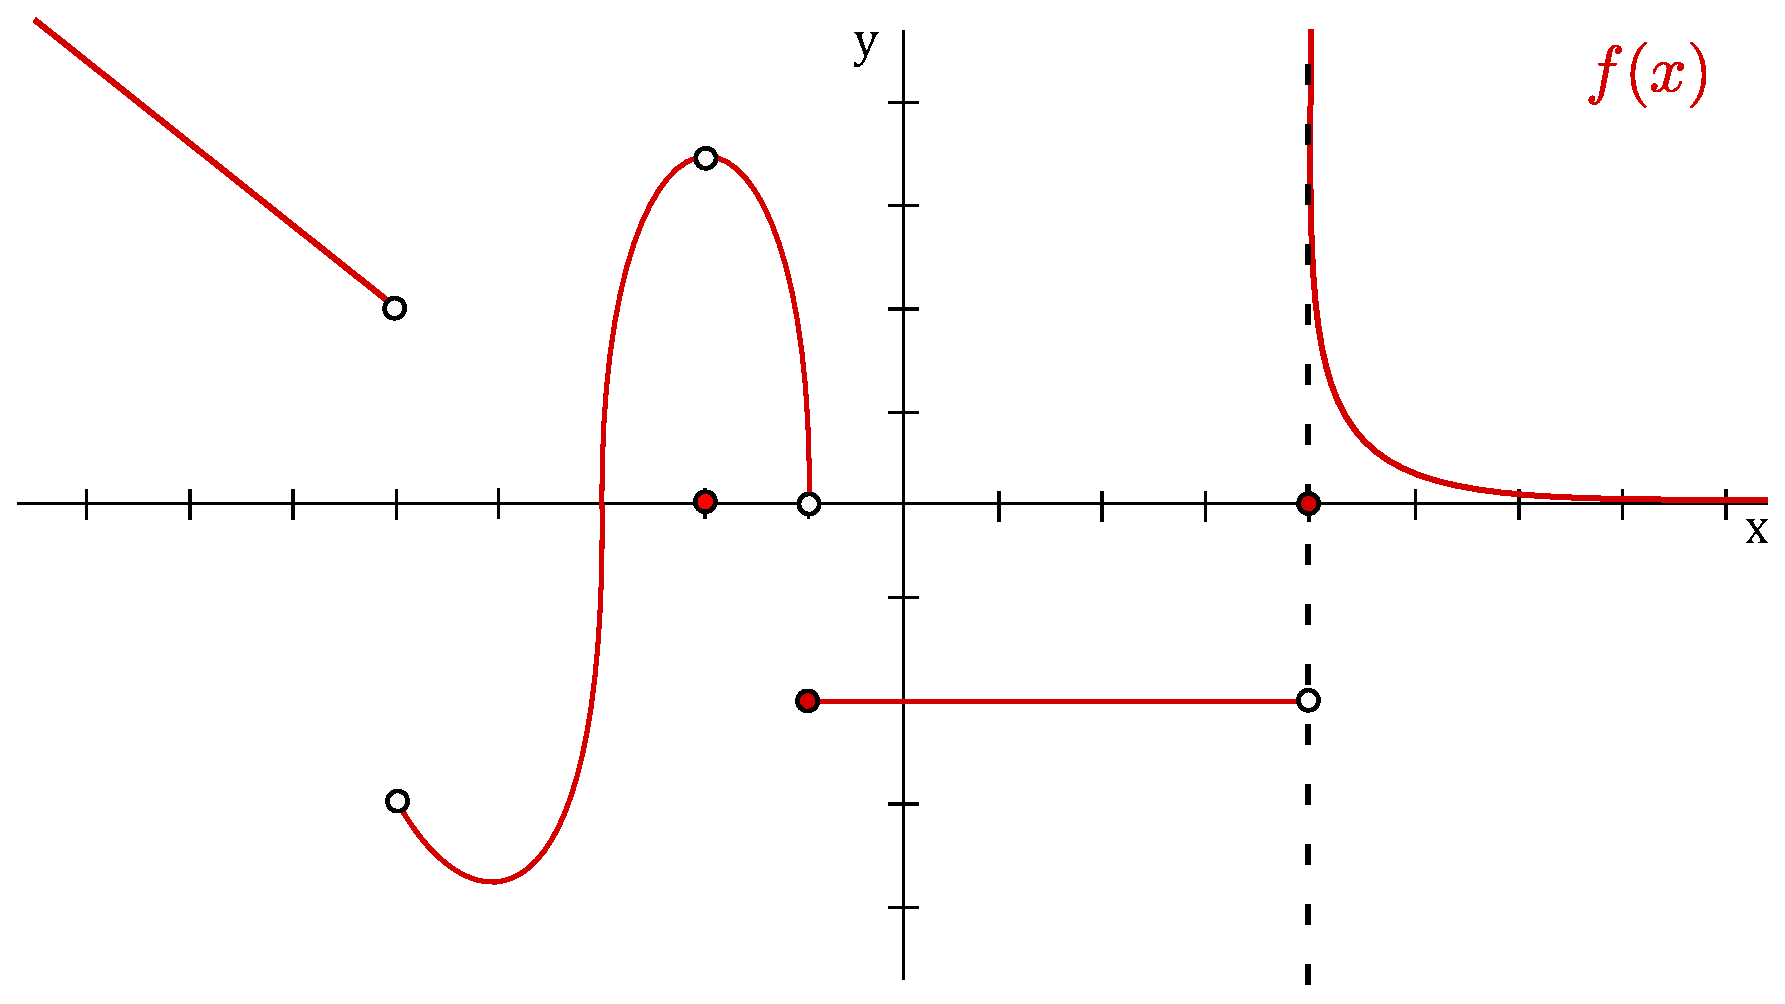
\includegraphics[width=5.5in]{images/limits-graphically}$$

Observe that $f(x)$ is indeed a function (it passes the vertical line test). We now analyze the function at each point separately.

$\ifont{x=-5:}$ Observe that at $x=-5$ there is no closed circle, thus $f(-5)$ is undefined.
From the graph we see that as $x$ gets closer and closer to $-5$ from the left, then $f(x)$ approaches $2$, so
$$\lim_{x\to -5^-}f(x)=2.$$
Similarly, as $x$ gets closer and closer $-5$ from the right, then $f(x)$ approaches $-3$, so
$$\lim_{x\to -5^+}f(x)=-3.$$
As the right-hand limit and left-hand limit are not equal at $-5$, we know that
$$\lim_{x\to -5}f(x)\quad\mbox{does not exist.}$$

$\ifont{x=-2:}$ Observe that at $x=-2$ there is a closed circle at $0$, thus $f(-2)=0$.
From the graph we see that as $x$ gets closer and closer to $-2$ from the left, then $f(x)$ approaches $3.5$, so
$$\lim_{x\to -2^-}f(x)=3.5.$$
Similarly, as $x$ gets closer and closer $-2$ from the right, then $f(x)$ again approaches $3.5$, so
$$\lim_{x\to -2^+}f(x)=3.5.$$
As the right-hand limit and left-hand limit are both equal to $3.5$, we know that
$$\lim_{x\to -2}f(x)=3.5.$$

Do not be concerned that the limit does not equal 0. This is a discontinuity, which is completely valid, and will be discussed in a later section.

We leave it to the reader to analyze the behaviour of $f(x)$ for $x$ close to $-1$ and $0$.
 
Summarizing, we have:
\hspace{-2.3cm}{
$$\begin{array}{|c|c|c|c|}
\hline&~&~&~\\
f(-5)~\mbox{is undefined} & f(-2)=0 & f(-1)=-2 & f(0)=-2  \\
~&~&~&~\\
\ds{\lim_{x\to -5^-}f(x)=2} & \ds{\lim_{x\to -2^-}f(x)=3.5} & \ds{\lim_{x\to -1^-}f(x)=0} & \ds{\lim_{x\to 0^-}f(x)=-2}  \\
~&~&~&~\\
\ds{\lim_{x\to -5^+}f(x)=-3} & \ds{\lim_{x\to -2^+}f(x)=3.5} & \ds{\lim_{x\to -1^+}f(x)=-2} & \ds{\lim_{x\to 0^+}f(x)=-2}\\
~&~&~&~\\
\ds{\lim_{x\to -5}f(x)=\mbox{DNE}} & \ds{\lim_{x\to -2}f(x)=3.5} & \ds{\lim_{x\to -1}f(x)=\mbox{DNE}} & \ds{\lim_{x\to 0}f(x)=-2}\\
~&~&~&~\\
\hline
\end{array}$$
}
%\end{solution}


%%%%%%%%%%%%%%%%%%%%%%%%%%%%%%%%%%%%%%%%%%%%
\Opensolutionfile{solutions}[ex]
\section*{Exercises for Section \ref{sec:LimitsGraphically}}

\begin{enumialphparenastyle}

%%%%%%%%%%
\begin{ex}
Evaluate the expressions by reference to this graph:
$$\includegraphics[width=3.5in]{images/limit-exercise-graph}$$
\begin{multicols}{3}
\begin{enumerate}
	\item	$\ds \lim_{x\to 4} f(x)$
	\item	$\ds \lim_{x\to -3} f(x)$
	\item	$\ds \lim_{x\to 0} f(x)$
	\item	$\ds \lim_{x\to 0^-} f(x)$
	\item	$\ds \lim_{x\to 0^+} f(x)$
	\item	$\ds f(-2)$
	\item	$\ds \lim_{x\to 2^-} f(x)$
	\item	$\ds \lim_{x\to -2^-} f(x)$
	\item	$\ds \lim_{x\to 0} f(x+1)$
	\item	$\ds f(0)$
	\item	$\ds \lim_{x\to 1^-} f(x-4)$
	\item	$\ds \lim_{x\to 0^+} f(x-2)$
\end{enumerate}
\end{multicols}
\begin{sol}
\begin{multicols}{3}
\begin{enumerate}
	\item	$8$
	\item	$6$
	\item	dne
	\item	$-2$
	\item	$-1$
	\item	$8$
	\item	$7$
	\item	$6$
	\item	$3$
	\item	$-3/2$
	\item	$6$
	\item	$2$
\end{enumerate}
\end{multicols}
\end{sol}
\end{ex}

\end{enumialphparenastyle}